% !TEX root=../../Thesis.tex
\newcommand {\matr}[2]{\left[\begin{array}{#1}#2\end{array}\right]}
\newcommand{\E}{\mathbb{E}}
\newcommand{\tr}{\mathrm{tr}}
\newcommand{\x}{{\mathbf{x}}}
\renewcommand{\u}{{\mathbf{u}}}
\newcommand{\w}{{\mathbf{w}}}
\renewcommand{\r}{{\mathbf{r}}}

\chapter{Modeling Intersection Driving Scenarios}
\label{ch:modeling_intersection}
% \begin{center}
%   \textit{\textbf{RQ 1: How can \gls{rl} be used to create a decision-making agent for driving through intersections?}}
% \end{center}
%   \vspace{12pt}

Navigating an intersection is a sequential decision-making problem that can be mathematically modeled using a \gls{mdp}, as introduced in Section~\ref{sec:background_mdp}. This thesis focuses on driving through intersections in the presence of other drivers, emphasizing not only to follow traffic rules but also the ability to adapt to the intentions of other drivers. Given that current sensors cannot directly observe other drivers' intentions, a \gls{pomdp} is a more suitable framework for formulating this problem.

\section{POMDP formulation}
\label{sec:pomdp_fomulation}
Effectively modeling the intersection problem is key for developing an optimal decision-making policy. While specific details of the \gls{pomdp} may vary between different studies, the general description remains consistent. This section outlines the essential aspects of the \gls{pomdp} framework as applied to the intersection problem in this thesis.

\subsection{State space}
\label{sec:pomdp_statespace}

\begin{figure}[h]
	\centering
	\begin{tikzpicture}
	
		% Crossing
		\def\crosstopy{5}
		\def\crossboty{-2.5}
		\def\crossleftx{-5}
		
		\draw[thick] (\crossleftx, 1) -- (-1, 1) -- (-1, \crosstopy);
		\draw[thick] (\crossleftx, -1) -- (-1, -1) -- (-1, \crossboty);
		\draw[thick] (1, \crosstopy) -- (1, 1) -- (3, 1);
		\draw[thick] (1, \crossboty) -- (1, -1) -- (3, -1);
		
		cars
		\node[inner sep=0pt] (ego_car) at (-4,0)
		{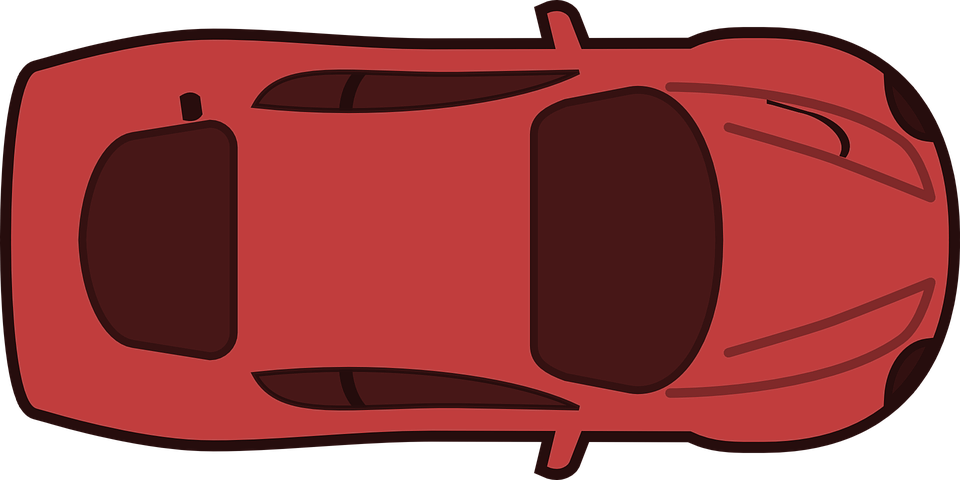
\includegraphics[width=.18\textwidth, angle=0]{figures/ego_car_top_down.png}};
		\draw[->] ([yshift=0.2cm]ego_car.east) -- node[above] {$p_\mathrm{ego}, v_\mathrm{ego}$} ($ (ego_car) + (2.5,0.2)$ );
		% \draw[|-|] ([yshift=-0.2cm]ego_car.east) -- node[below] {$p_{ego}$} (-1,-0.2);
	
		% \node[inner sep=0pt] (target_car_3) at (0,7)
		% {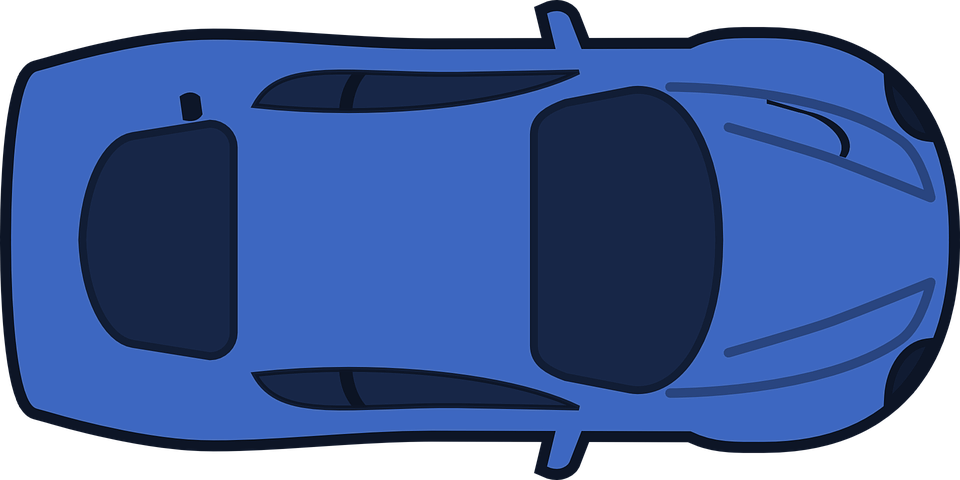
\includegraphics[width=.18\textwidth, angle=-90]{figures/target_car_top_down.png}};
		% \node (tc_text3a) [right=of target_car_3, align=center] {Car $n$};
		% % \node (tc_text3b) [left=of target_car_3, align=center] {Conflict Car};
		% \draw[->] ([xshift=-.3cm]target_car_3.south) -- node[right] {$p_{n} v_{n} \zeta_n$} ($ (target_car_3) + (-.3,-2)$ );
		% \draw[|-|] ([xshift=-0.8cm]target_car_3.south) -- (-.8,1);
		% \node (tc_tti) [below left= 0.9cm and -0.7cm of target_car_3, align=center] {$p_n$  \\ $\tau_{int}$};
	
		\node[inner sep=0pt] (target_car_2) at (0,3.5)
		{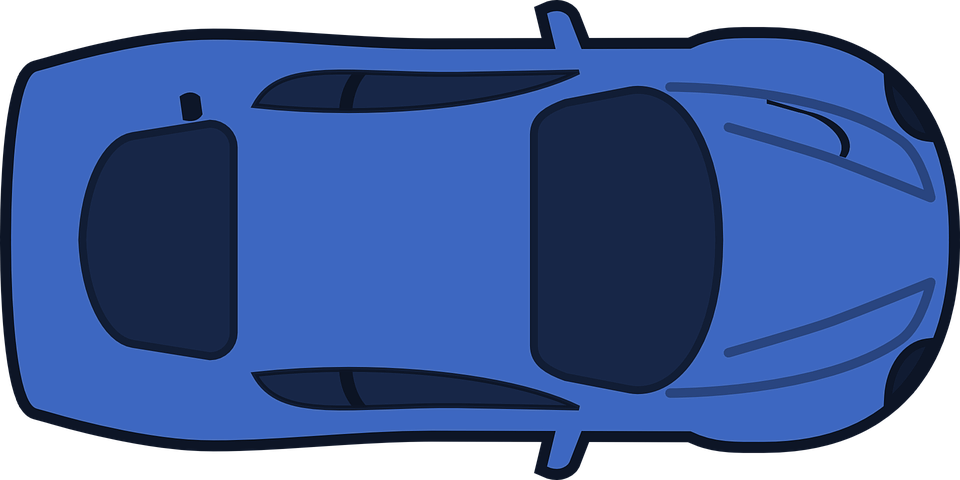
\includegraphics[width=.18\textwidth, angle=-90]{figures/target_car_top_down.png}};
		\node (tc_text2) [right=of target_car_2] {Car $n$};
		\draw[->] ([xshift=-.3cm]target_car_2.south) -- node[right] {$p_{n} v_{n} \zeta_n$} ($ (target_car_2) + (-.3,-2)$ );
		
		\node[inner sep=0pt] (target_car_1) at (0,-1.5)
		{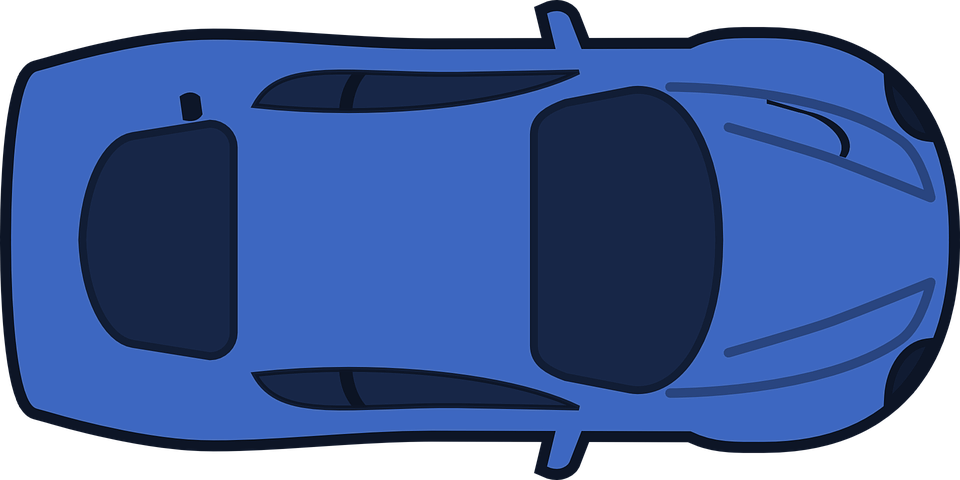
\includegraphics[width=.18\textwidth, angle=-90]{figures/target_car_top_down.png}};
		\node (tc_text1) [right=of target_car_1] {Car 1};
	
	\end{tikzpicture}
	\caption{General description of the states in a simple intersection. The ego vehicle in red is controlled by the agent, while the blue vehicles are the other vehicles crossing the same intersection. Each blue vehicle is described by an index $n$, a position $p_n$, a velocity $v_n$  and hidden intention $\zeta_n$}.
	\label{fig:intersection_scenario}
	\end{figure}

From Section~\ref{sec:background_mdp}, the state space contains all the information necessary about the agent and environment to be able to transition from any given state $s$ to the next state $s'$. In the scenario shown in Figure~\ref{fig:intersection_scenario}, the red car on the horizontal lane represents the ego vehicle controlled by the agent while the blue cars on the vertical lane are the other vehicles which ego needs to interact with in order to cross the intersection. 

A simplified description of the state, 
\begin{align}
	s = (p_\mathrm{ego}, v_\mathrm{ego}, \{p_{n}, v_n, \zeta_n\}_{n=1}^N), 
	\label{eq:state}
\end{align}
consists of positions state $p_\mathrm{ego}$ and $p_n$, where subscript \textit(ego) and $n$ denotes ego vehicle and the index of the surrounding vehicle up to $N$ vehicles. 
% Let's start by defining the information needed. 
Instead of using a Cartesian coordinate system to describe the position $p_\mathrm{ego}$ and $p_n$, relative distance measures are proposed instead. This way, the state space are generalizable to different intersection designs, e.g., the angle of incidence and number of crossing points. 
The velocity of ego $v_\mathrm{ego}$ and all other the traffic participants $v_n$ is also necessary to be able to predict what position they will be in the next state. Finally, the intention of all the other participants $\zeta_n$. As mentioned in Section \ref{sec:intro_intersections}, $\zeta_n$ encapsules information such as stop sign, traffic light or even inattention in to one state. 
\paperBelief \ shows a comparison between two fully observable \gls{mdp}s, one with intention and the other one without and the results show that having an intention state reduce number of collisions. 
\paperLSTM \ used a \gls{lstm} network architecture to implicitly predict $\zeta$. %The states describing ego and other vehicle are spearated. Repeat the states for each other vehicle we observe. 

\subsection{Action space}
\label{sec:pomdp_actionspace}
One limitation of deep Q-learning is the requirement for a discrete action space. In various \gls{ad} studies \cite{bouton2019}, it is common practice to define the action space in terms of different acceleration requests. The approach in \paperLSTM \ proposes using short-term goals as actions: \{\textit{`take way', `yield', `follow car~$\{1, \dots , N\}$'}\}.

These short-term goals represent high-level objectives, such as driving through an intersection (take way), stopping at the start of an intersection (yield) or drive behind a specific car (follow car~$n$). Each high-level action is translated into a set of parameters that are input into a sliding mode controller in \paperLSTM \ and a \gls{mpc} in \paperMPC, which then generates the appropriate acceleration to control the ego car.

\subsection{Transition model}
\label{sec:pomdp_transistionmodel}
The transition model is initially unknown, and \gls{rl} is employed to learn this model by taking actions in the environment from different states, recording the resulting rewards, and noting the subsequent state transitions. In this work, the environment is a simulator, and the primary objective for the agent is to learn the transition dynamics of other vehicles, which depend on their intentions $\zeta$. These intentions are modeled as predetermined actions, governed by an \gls{idm}. Using the \gls{idm} to guide predetermined actions makes the interactions between vehicles more complex, which complicates the learning process. For more details on the simulation environment see Chapter~\ref{ch:simulation_env}.


\subsection{Observation model}
The observation space typically mirrors the state space, excluding the intention state $\zeta$, as there are no sensors capable of directly detecting other drivers' intentions. This observation 
\begin{align}
	o = (p_\mathrm{ego}, v_\mathrm{ego}, \{p_{n}, v_n\}_{n=1}^N), 
	\label{eq:observation}
\end{align}
encompasses all elements of the state space, from \eqref{eq:state}, that are observable through the sensors in the car, except for the intention state $\zeta$.

\subsection{Reward function}
The design of the reward function is pivotal as it determines the value associated with each state, ultimately shaping the driving policy of the agent. A well-crafted reward function is instrumental in guiding the agent towards achieving its objectives effectively.
The reward model in this work is formulated based on terminal states, including reaching the goal, collision events, and timeouts. These terminal states play a critical role in defining the success or failure of the agent's driving behavior and are accordingly reflected in the reward structure.

\section{Simulation environment}
\label{ch:simulation_env}
The simulation environment in this thesis, first introduced in \paperLSTM, places an agent at an intersection tasked with reaching the goal across the intersection while interacting with up to $N$ other cars on the intersecting lane. At the beginning of each episode, up to $N$ vehicles are initialized with initial positions $p_n^0$ distributed along the intersecting lane, starting velocities $v_n^0$ and a deterministic policy that defines their intention $\zeta_n$. 
Each vehicle, including the ego vehicle, adheres to the \gls{idm} (Section~\ref{ch:idm}) aimed at maintaining specific speeds and safe distances, with the maximum acceleration is capped at $5 m/s^2$ to ensure comfort and safety under normal driving conditions.
For example, if a vehicle's intention $\zeta_n$ is yield, it would set the \gls{idm} for the distance to the object in front  $d_n$ to the distance to the start of the intersection, and its velocity $v_{n-1}$ would be set to $0$. Alternatively, a vehicle with a take way intention would follow the IDM only considering the vehicle directly in front of it.

During the simulation, whenever a vehicle in the perpendicular lane crosses the intersection, it is removed from the environment. Subsequently, a new vehicle is spawned at the start of that lane at a random time, with new initial values for position $p_n^0$, velocity $v_n^0$, desired velocity $v^\mathrm{desired}_n$ and intention $\zeta_n$. 
This dynamic spawning process ensures that the traffic scenario continually evolves, presenting varying challenges and interactions for the agent navigating the intersection.
Each episode continues until a terminal state is reached, which can be a reaching the goal, collision, safe stop, or deadlock. Rewards are assigned based on a predefined reward function designed to reinforce desired behaviors.


\section{Deep Q-learning approach}
To find a driving policy $\pi$ for the \gls{pomdp} detailed in the previous section, both \paperLSTM \ and \paperMPC \ used deep Q-learning, described Chapter~\ref{ch:q-learning}. \paperLSTM \ proposed a \gls{dqn} structure with shared weights and \gls{lstm} layer to approximate the Q-function. Because the scenarios has up to $N$ cars that with same type of states, the shared weight is an effective way to reduce the input space the agent need to explore. While the \gls{lstm} layer has the role of utilizing the previous states to implicitly estimate a hidden state that could possibly encapsulate the intention of other cars.

As mentioned in Chapter~\ref{sec:pomdp_actionspace}, the actions in \paperLSTM \ are controlled by a sliding mode controller while \paperMPC \ use a \gls{mpc} to generate a velocity profile for a short time horizon. Instead of specifying which car to drive behind, the action in this context determines which gap between cars the vehicle should drive through. This gap is then translated into constraints that the \gls{mpc} uses to create the velocity profile.

\gls{mpc} excels at creating plans within given constraints but faces challenges with mixed integer problems, making the calculation of the optimal path for all possible actions computationally intensive. On the other hand, Q-learning is effective at estimating the value of an action given a state, but it requires exploring many suboptimal actions before converging on a good one. By combining \gls{rl} and \gls{mpc}, an agent can efficiently select a good action, which the \gls{mpc} can then use to generate a safe and efficient velocity profile.

The agents from \paperLSTM \ and \paperMPC \ are evaluated on both a single intersection, shown in Figure~\ref{fig:example_intersections}\subref{fig:single_intersection}, and a double intersection with two crossing points, shown in Figure~\ref{fig:example_intersections}\subref{fig:double_intersection}. The results are summarized in Table~\ref{tab:results_single_double_crossing}.

\section{Results from simulation}
\label{sec:results_dqn}
The results from Table~\ref{tab:results_single_double_crossing} showed that the proposed \gls{dqn} agent from \paperLSTM \ found a policy that successfully crossed a single intersection $96.1\%$ of the time, with $2.8\%$ resulting in collisions and $1.1\%$ resulting in timeouts. 
When comparing agents trained with and without an \gls{lstm} layer, those with the \gls{lstm} succeeded in 3 out of 4 attempts where those without it would fail.
This demonstrates that deep Q-learning has great potential for creating decision-making agents capable of navigating intersections. Additionally, the results from Figure~\ref{fig:results_shared} indicate that using a network structure with shared weights between cars significantly improved the convergence speed of the network. Shared weights, along with other enhancements like dropout and experience replay, are essential components for this improvement.

\begin{figure}[!ht]
	\centering
	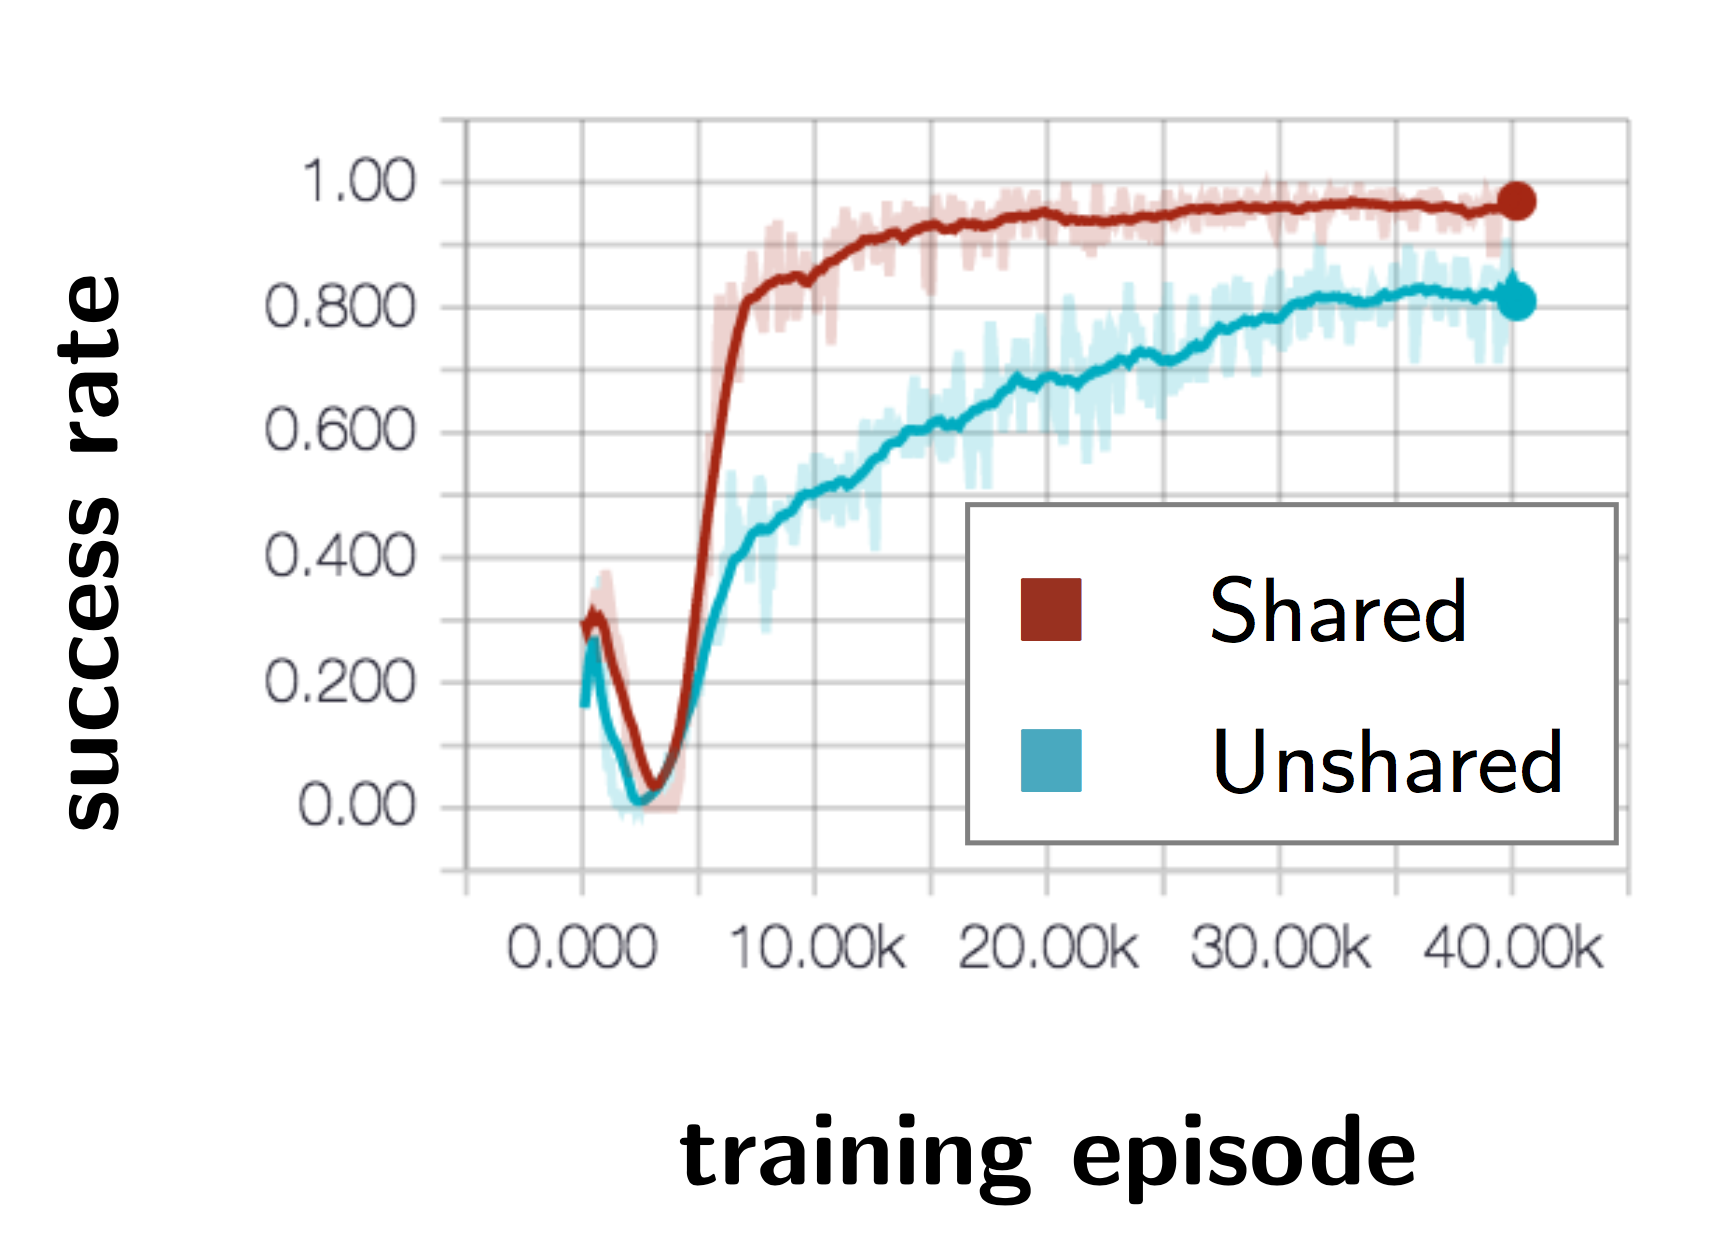
\includegraphics[width=0.7\columnwidth]{YourThesis/papers/lstm/figures/results_shared.png}
	\caption{The figure shows that the success rate for a network with shared weights (brown line) converge faster than the fully connected network structure which do not share weights (turquoise line).}
	\label{fig:results_shared}
\end{figure}

As mentioned previously, the controller from \paperLSTM \ could only consider one car at a time, which placed a heavy burden on the \gls{dqn} compensate by frequently switching actions. 
In contrast, in \paperMPC, the \gls{mpc} showed significant improvement in handling more complex intersections.
For instance, in the double intersection, the \gls{mpc} agent succeeded $95.2\%$ of the time with a collision rate of $3.6\%$, compared to the sliding mode controller, which only succeeded $90.9\%$ of the time with a collision rate of $8.3\%$.


% \begin{figure}[!ht]
% 	\centering
% 	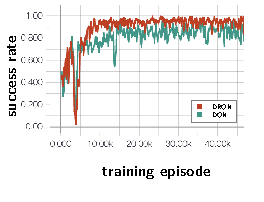
\includegraphics[width=0.7\columnwidth]{figures/figures-recurrent.pdf}
% 	\vspace{-0.5cm}
% 	\caption{Graphs presenting the performance of a DRQN (red) compared to a DQN with a single observation (green), running on scenarios with cars that have different behaviors. When compared a DRQN succeeds in 3 out of 4 attempts, where a DQN fails.}
% 	\label{fig:results_recurremt}
% \end{figure}

% \begin{figure}[t!]
	% \mbox{\parbox{\textwidth}{
% 	\centering
% 	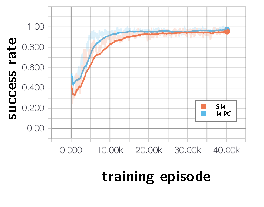
\includegraphics[width=\columnwidth]{YourThesis/papers/mpc/figures/figures-successrate.pdf}
% }}
% 	\caption{Average MPC and SM success rate for a single corssing after evaluating the policy 300 episodes.}
% 	\label{fig:result1}
% \end{figure}

% \begin{figure}[t!]
% 	\centering
% 	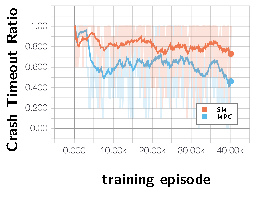
\includegraphics[width=\columnwidth]{YourThesis/papers/mpc/figures/figures-crashratio.pdf}
% 	\vspace{-4em}
% 	\caption{Average MPC and SM crash to timeout ratio for a single crossing after evaluating the policy in 300 episodes. A CTR of $0$ means that all failures are timeouts, while a CTR of $1$ means that all failures are collisions.}
% 	\label{fig:result2}
% \end{figure}

\begin{table}[h]
	\mbox{\parbox{\textwidth}{
	\centering
	\begin{tabular}{ |p{2,6cm}||p{1,2cm}|p{1,2cm}|p{1,2cm}|p{1,2cm}|}
	\hline
	Controller &\multicolumn{2}{|c|}{Success Rate}&\multicolumn{2}{|c|}{Collision Rate}\\
	\hline
	 & Single & Double & Single & Double\\
	\hline
	SM (\paperLSTM) & $96.1\%$ & $90.9\%$ & $2.8\%$ & $8.3\%$\\
	MPC (\paperMPC) & $97.3\%$ & $95.2\%$ & $1.2\%$ & $3.6\%$\\
	\hline
	\end{tabular}
	}}
	\caption{Average success rates and collision rates for a fully trained \gls{dqn} agent driving through a single and double intersections. If the agent failed to reach the goal or collide within a given time, the terminal state was classified as a timeout.}% across single and double crossings.}   
\label{tab:results_single_double_crossing}
\end{table}


\section{Discussion}
% \section{The intersection problem}
\begin{figure}
	\mbox{\parbox{\textwidth}{
		\centering
		\begin{tikzpicture}
			\def\xstart{-7};

			\coordinate (p) at (3,0);
			\foreach \n/\w/\c in {z0/2/green,z1/2/red,z2/2.5/orange,z3/3.5/blue}{
				\node[rectangle,
				draw=none,
				anchor=east,
				text = black,
				fill = \c!60,
				minimum width = \w cm, 
				minimum height = 2cm] 
				(n) at (p) {\Huge \n};
				
				\coordinate (p) at (n.west);
			}

			% Crossing
			\draw[line width=0.5mm] (\xstart, 1) -- (-1, 1) -- (-1, 5);
			\draw[line width=0.5mm] (\xstart, -1) -- (-1, -1) -- (-1, -2);
			\draw[line width=0.5mm] (1, 5) -- (1, 1) -- (3, 1);
			\draw[line width=0.5mm] (1, -2) -- (1, -1) -- (3, -1);
			
			% cars
			\node[inner sep=0pt] (ego_car) at (-7,0)
			{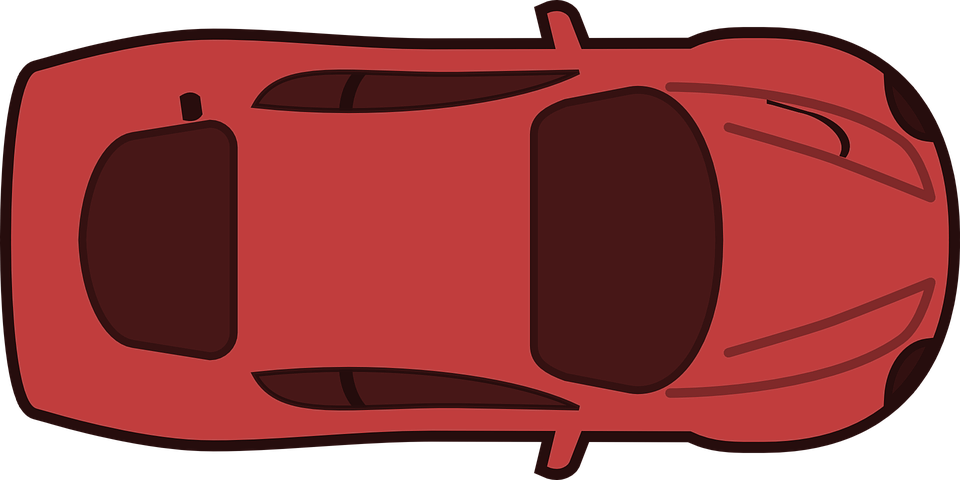
\includegraphics[width=.18\textwidth, angle=0]{figures/ego_car_top_down.png}};
			\node[inner sep=0pt] (target_car) at (0,4)
			{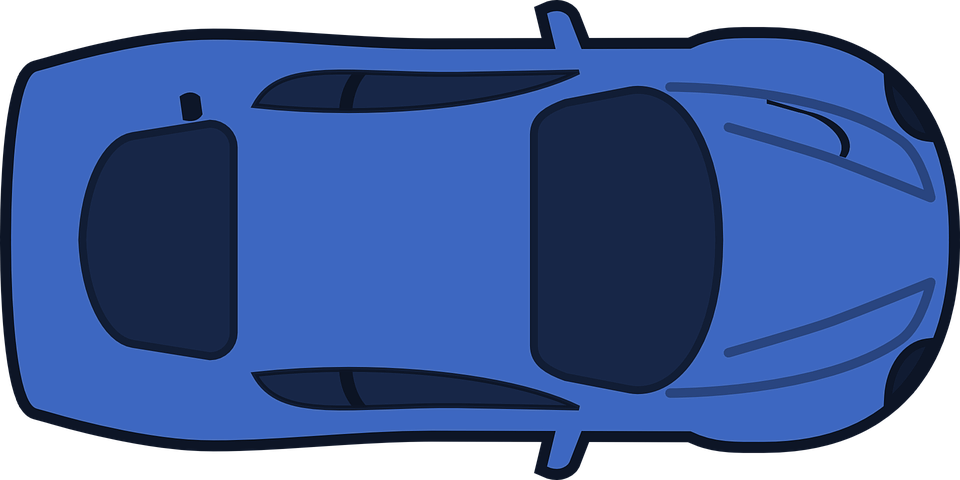
\includegraphics[width=.18\textwidth, angle=-90]{figures/target_car_top_down.png}};

	\end{tikzpicture}
	}}
	\caption{Intersection scenario divided into zones describing what is required of the decision maker in different zones}
	\label{fig:zones}
\end{figure}

Observing the behavior of a fully trained agent from \paperLSTM \ and \paperMPC \ provides the insight that the path of the ego vehicle can be segmented into four zones, illustrated in Figure~\ref{fig:zones}. Starting from the right, Zone 0 represents the 'safe zone,' where the ego vehicle is out of danger and can resume nominal driving. Zone 1 is the 'conflict zone,' where a collision with another vehicle is possible. Zone 2, the 'critical decision zone,' is the final opportunity for the vehicle to either stop or proceed through the intersection. The size of zone 2 is determined by the minimum distance required for the vehicle to come to a complete stop before entering the conflict zone, ensuring sufficient time for safe decision-making. Lastly, Zone 3, the 'information gathering zone,' is situated furthest from the intersection. Here, the agent can observe how other vehicles behave over time to estimate their intentions.

The goal is to reach Zone 0. To achieve this, the agent aims to minimize the time spent in Zone 1 if there is a chance of intersection with another car. Our actions are formulated as short-term goals, designed for comfortable use with lower acceleration rates. The size of Zone 2 depends on the vehicle's current speed, which is influenced by its behavior in Zone 3.

Now, two conflicting strategies emerge: to minimize time in Zone 1, the agent desires a high speed entering the intersection. However, it also seeks a low speed to reduce the size of Zone 2 and the critical decision period. If the intentions of other vehicles are known, the stochasticity in Zone 1 would be eliminated, transforming the problem into a scheduling task aimed at creating a velocity profile that minimizes the time required to cross. However, since the intentions of other vehicles are inherently stochastic, the next chapter offers a promising approach by accounting for this uncertainty and optimizing decision-making in dynamic traffic scenarios.


